\model{Circle objects}
\label{CS1/class-circle}

Unified Modeling Language (UML) provides a way of graphically illustrating a class’s design, independent of the programming language.

\begin{center}
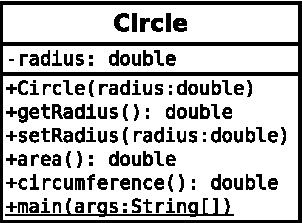
\includegraphics{CS1/Circle.pdf}
\end{center}


\quest{15 min}


\Q What are the attributes and methods of \java{Circle}, and what is their \emph{visibility}?

\begin{answer}
The attribute \java{radius} is private, and the methods \java{Circle}, \java{area}, \java{circumference}, \java{getRadius}, and \java{setRadius} are public.
\end{answer}


\Q Based on \ref{CS1/class-die} and \ref{CS1/class-circle}, what is typically \java{public} and what is typically \java{private}?

\begin{answer}
Attributes are typically private, and methods are typically public.
\end{answer}


\Q How would you declare a variable named \java{unit} that is a \java{Circle} object?
How would you instantiate a circle with a radius of 1.0 and assign it to \java{unit}?

\begin{answer}
\tt Circle unit;

\tt unit = new Circle(1.0);
\end{answer}


\Q Write the code (inside {\tt Circle.java}) that declares the \java{radius} attribute.

\begin{answer}
\tt private double radius;
\end{answer}


\Q Write the code for \java{getRadius}. (Don't worry about Javadoc comments for this activity.)

\begin{answer}[6em]
\begin{javaans}
    public double getRadius() {
        return radius;
    }
\end{javaans}
\end{answer}


\Q Write the code for \java{setRadius}. Note there are two variables named \java{radius}: the parameter of \java{setRadius}, and \java{this.radius} for the object itself. Before you set the radius, first check if the parameter is negative, and if it is, set \java{this.radius} to zero instead.

\begin{answer}[12em]
\begin{javaans}
    public void setRadius(double radius) {
        if (radius >= 0) {
            this.radius = radius;
        }
        else {
            this.radius = 0;
        }
    }
\end{javaans}
\end{answer}


\Q Write the complete code for \java{area} and \java{circumference}.
The area of a circle is $\pi r^2$, and the circumference is $2 \pi r$.
Ideally, each method should be one line of code.

\begin{answer}[12em]
\begin{javaans}
    public double area() {
        return Math.PI * radius * radius;
    }

    public double circumference() {
        return 2.0 * Math.PI * radius;
    }
\end{javaans}
\end{answer}


\Q Write a \java{main} method that creates a \java{Circle} object with a radius of 2.0 and displays its area and circumference on the screen.

\begin{answer}[8em]
\begin{javaans}
    public static void main(String[] args) {
        Circle big = new Circle(2.0);
        System.out.println("big area = " + big.area());
        System.out.println("big circ = " + big.circumference());
    }
\end{javaans}
\end{answer}
